%%%%%%%%%%%%%%%%%%%%%%%%%%%%%%%%%%%%%%%%%%%%%%%%%%%%%
% Primary document settings
%%%%%%%%%%%%%%%%%%%%%%%%%%%%%%%%%%%%%%%%%%%%%%%%%%%%%

\documentclass[aspectratio=169,12pt]{beamer}

\usepackage{ifxetex,ifluatex}
\ifnum 0\ifxetex 1\fi\ifluatex 1\fi=0 % if pdftex
  \usepackage[T1]{fontenc}
  \usepackage[utf8]{inputenc}
  \usepackage{textcomp} % provide euro and other symbols
\else % if luatex or xetex
  \usepackage{unicode-math}
  \defaultfontfeatures{Scale=MatchLowercase}
  \defaultfontfeatures[\rmfamily]{Ligatures=TeX,Scale=1}

\usepackage[
    backend=biber,
    natbib=true,
    style=authoryear-comp,
    %bibstyle=authoryear,
    %autocite=footnote,
    %style=authoryear,
    sorting=nyt,
    %sortlocale=de_DE,
    sortlocale=en_US,
    url=false,
    doi=true,
]{biblatex}

\addbibresource{references.bib}

\usepackage{fancyqr}

%%%%%%%%%%%%%%%%%%%%%%%%%%%%%%%%%%%%%%%%%%%%%%%%%%%%%%%%%%%%%%
% Extra stuff for Rmarkdown to work (code blocks)
%%%%%%%%%%%%%%%%%%%%%%%%%%%%%%%%%%%%%%%%%%%%%%%%%%%%%%%%%%%%%%
\providecommand{\tightlist}{%
  \setlength{\itemsep}{2pt}\setlength{\parskip}{0pt}}

\usepackage{graphicx}
\makeatletter
% New in pandoc https://github.com/jgm/pandoc-templates/commit/6c0e7b0a4f990debcd38b5c3bd8599193ae8f5a6#diff-f218051b4ca8f740a9f585a149101d4a3025037c568b391b5216edf7b14cfadc
\newsavebox\pandoc@box
\newcommand*\pandocbounded[1]{% scales image to fit in text height/width
\sbox\pandoc@box{#1}%
\Gscale@div\@tempa{\textheight}{\dimexpr\ht\pandoc@box+\dp\pandoc@box\relax}%
\Gscale@div\@tempb{\linewidth}{\wd\pandoc@box}%
\ifdim\@tempb\p@<\@tempa\p@\let\@tempa\@tempb\fi% select the smaller of both
\ifdim\@tempa\p@<\p@\scalebox{\@tempa}{\usebox\pandoc@box}%
\else\usebox{\pandoc@box}%
\fi%
}
% Set default figure placement to htbp
\def\fps@figure{htbp}
\makeatother

%%%%%%%%%%%%%%%%%%%%%%%%%%
% kableExtra stuff (tables)
%%%%%%%%%%%%%%%%%%%%%%%%%%
\usepackage{booktabs}
\usepackage{longtable}
\usepackage{array}
\usepackage{multirow}
\usepackage{xcolor}
\usepackage{wrapfig}
\usepackage{float}
\usepackage{colortbl}
\usepackage{pdflscape}
\usepackage{tabu}
\usepackage{threeparttable}
\usepackage{threeparttablex}
\usepackage[normalem]{ulem}
\usepackage{makecell}



%%%%%%%%%%%%%%%%%%%%%%%%%%
% Main document
%%%%%%%%%%%%%%%%%%%%%%%%%%

\usetheme[]{BIPS}
%\usetheme[german]{BIPS}  % for the German version
%\usetheme[fira]{BIPS} % English with the Fira font
%\usetheme[german,fira]{BIPS} % German with the Fira font

% Note that for the Fira font, you need to use
% XeLaTeX instead of pdfLaTeX. You can find this in
% most interfaces

\title{Random Planted Forest:\\
A Directly Interpretable Tree Ensemble}
\subtitle{}
\author{Meyer, J. T.\inst{5} \and Burk, L.\inst{1,2,3,4} \and Hiabu,
M.\inst{6} \and Mammen, E.\inst{5}}
\date{}
\contactauthor{Lukas Burk}
\occasion{DAGStat 2025 --- March 27th, 2025}
\email{burk@leibniz-bips.de}
\institute{\textsuperscript{1}Leibniz Institute for Prevention Research
and Epidemiology -- BIPS \and \textsuperscript{2}LMU Munich
\quad \textsuperscript{3}University of
Bremen \and \textsuperscript{4}Munich Center for Machine Learning
(MCML) \and \textsuperscript{5}Heidelberg University
\quad \textsuperscript{6}University of Copenhagen}


%%% Title Page
\setbeamertemplate{title page}{
	\usebeamercolor{title page}
	\begin{tikzpicture}
		\useasboundingbox (1,0) rectangle (\the\paperwidth,\the\paperheight);
		\node[font=\usebeamerfont{title}, color=BIPSBlue, text width=14cm, align=center] at (\paperwidth*.5,7) {\inserttitle} ;
		% \node[align=center, font=\usebeamerfont{subtitle}, color=BIPSBlue] at (\paperwidth*.5, 5.5) {\insertsubtitle};
		\node[align=center, font=\usebeamerfont{author}, color=BIPSBlue] at (\paperwidth*.5, 5) {\insertauthor};
		\node[align=center, font=\usebeamerfont{institute}, color=BIPSTextGray] at (\paperwidth*.5, 3) {\textsuperscript{1}Leibniz
Institute for Prevention Research and Epidemiology --
BIPS \\ \textsuperscript{2}LMU Munich
\quad \textsuperscript{3}University of
Bremen \\ \textsuperscript{4}Munich Center for Machine Learning
(MCML) \\ \textsuperscript{5}Heidelberg University
\quad \textsuperscript{6}University of Copenhagen};
		\node[align=center, font=\usebeamerfont{date}, color=BIPSTextGray] at (\paperwidth*.5, 1.5) {\insertdate};
		\node[align=center, font=\usebeamerfont{date}, color=BIPSTextGray] at (\paperwidth*.5, 1) {DAGStat
2025 --- March 27th, 2025};
	\end{tikzpicture}
}


\usepackage{tikz}
\usepackage{amsmath,amssymb}

\definecolor{brewer1}{rgb}{0.105882,0.619608,0.466667}
\definecolor{brewer2}{rgb}{0.85098,0.372549,0.00784314}
\definecolor{brewer3}{rgb}{0.458824,0.439216,0.701961}
\definecolor{brewer4}{rgb}{0.905882,0.160784,0.541176}

\usetikzlibrary{arrows.meta, shapes, positioning, calc}

\tikzset{
  root/.style={rectangle, rounded corners, minimum width=2cm, minimum height=0.8cm, text centered, draw=black, fill=brewer2, line width=1pt},
  internalnode/.style={rectangle, minimum width=1.7cm, minimum height=0.7cm, text centered, draw=black, fill=gray!2},
  decision/.style={ellipse, minimum width=1.7cm, minimum height=0.7cm, text centered, draw=black, fill=gray!2},
  rpfunique/.style={rectangle, minimum width=1.7cm, minimum height=0.7cm, text centered, draw=black, fill=brewer1},
  rpfuniquedecision/.style={ellipse, minimum width=1.7cm, minimum height=0.7cm, text centered, draw=black, fill=brewer1},
  interaction/.style={rectangle, minimum width=1.7cm, minimum height=0.7cm, text centered, draw=black, fill=brewer3},
  arrow/.style={thick,->,>=stealth},
  label/.style={font=\scriptsize}
}


\begin{document}
\addtocounter{framenumber}{-1}
\frame{\maketitle}

% \setcounter{framenumber}{1}


\begin{frame}{Motivation}
\phantomsection\label{motivation}
\begin{itemize}[<+->]
\tightlist
\item
  Tree-based methods like Random Forest (RF):

  \begin{itemize}[<+->]
  \tightlist
  \item
    Fast \& flexible
  \item
    Interpretable? → It depends
  \end{itemize}
\item
  Wishlist:

  \begin{itemize}[<+->]
  \tightlist
  \item
    Meaningful \emph{feature importance}
  \item
    Quantification of main- \emph{and interaction} \emph{effects}
  \end{itemize}
\item
  Additive models useful for both
\end{itemize}

\pause

\vfill

\begin{center}
→ \textbf{Random Planted Forest} (RPF): Additive Random Forest

\end{center}
\end{frame}

\begin{frame}{Functional ANOVA Expansion}
\phantomsection\label{functional-anova-expansion}
\begin{itemize}[<+->]
\tightlist
\item
  Regression with target \(Y_i \in \mathbb{R}\), features
  \(X_i \in \mathbb{R}^p\), instance \(\mathbf{x}_i\)
\item
  Expand prediction \(\hat{y}_i = \hat{m}(\mathbf{x}_i)\) into

  \begin{itemize}[<+->]
  \tightlist
  \item
    \(\hat{m}_{0}\): Average prediction (\emph{``intercept''})
    plus\ldots{}
  \item
    Terms \(\hat{m}_S\) with feature \(S \subseteq \{1, \ldots, p\}\)
  \end{itemize}
\end{itemize}

\pause

\vfill

\begin{align*}
\hat{m}(\mathbf{x}_i) = & \hat{m}_{0} + \\
&  \underbrace{\hat{m}_1(x_1) + \hat{m}_2(x_2) + \hat{m}_3(x_3)}_{\text{Main effect terms}} +
\end{align*}

\vfill
\end{frame}

\begin{frame}{Functional ANOVA Expansion}
\phantomsection\label{functional-anova-expansion-1}
\begin{itemize}
\tightlist
\item
  Regression with target \(Y_i \in \mathbb{R}\), features
  \(X_i \in \mathbb{R}^p\), instance \(\mathbf{x}_i\)
\item
  Expand prediction \(\hat{y}_i = \hat{m}(\mathbf{x}_i)\) into

  \begin{itemize}
  \tightlist
  \item
    \(\hat{m}_{0}\): Average prediction (\emph{``intercept''})
    plus\ldots{}
  \item
    Terms \(\hat{m}_S\) with feature \(S \subseteq \{1, \ldots, p\}\)
  \end{itemize}
\end{itemize}

\vfill

\begin{align*}
\hat{m}(\mathbf{x}_i) = & \hat{m}_{0} + \\
&  \underbrace{\hat{m}_1(x_1) + \hat{m}_2(x_2) + \hat{m}_3(x_3)}_{\text{Main effect terms}} + \\
&  \underbrace{\hat{m}_{1,2}(x_1,x_2) + \hat{m}_{1,3}(x_1,x_3) + \hat{m}_{2,3}(x_2,x_3)}_{\text{2nd order interactions}} +
\end{align*}

\vfill
\end{frame}

\begin{frame}{Functional ANOVA Expansion}
\phantomsection\label{functional-anova-expansion-2}
\begin{itemize}
\tightlist
\item
  Regression with target \(Y_i \in \mathbb{R}\), features
  \(X_i \in \mathbb{R}^p\), instance \(\mathbf{x}_i\)
\item
  Expand prediction \(\hat{y}_i = \hat{m}(\mathbf{x}_i)\) into

  \begin{itemize}
  \tightlist
  \item
    \(\hat{m}_{0}\): Average prediction (\emph{``intercept''})
  \item
    Terms \(\hat{m}_S\) with features \(S \subseteq \{1, \ldots, p\}\)
  \end{itemize}
\end{itemize}

\vfill

\begin{align*}
\hat{m}(\mathbf{x}_i) = & \hat{m}_{0} + \\
&  \underbrace{\hat{m}_1(x_1) + \hat{m}_2(x_2) + \hat{m}_3(x_3)}_{\text{Main effect terms}} + \\
&  \underbrace{\hat{m}_{1,2}(x_1,x_2) + \hat{m}_{1,3}(x_1,x_3) + \hat{m}_{2,3}(x_2,x_3)}_{\text{2nd order interactions}} + \\ 
&  \underbrace{\hat{m}_{1,2,3}(x_1,x_2,x_3)}_{\text{3rd order interaction}}
\end{align*}

\vfill
\end{frame}

\begin{frame}{Trees in Random Forest}
\phantomsection\label{trees-in-random-forest}
\begin{figure}[H]

{\centering 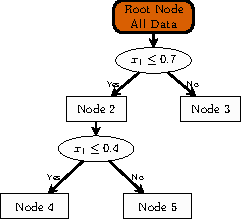
\includegraphics[width=\linewidth,height=0.75\textheight,keepaspectratio]{tree-cart.pdf}

}

\caption{CARTlike}

\end{figure}%
\end{frame}

\begin{frame}{Planted Trees (I)}
\phantomsection\label{planted-trees-i}
\begin{figure}

\centering{

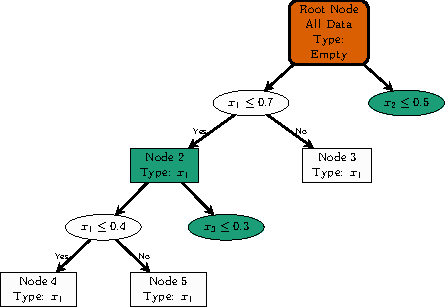
\includegraphics[width=\linewidth,height=0.75\textheight,keepaspectratio]{tree-planted-simple.pdf}

}

\caption{\label{fig-planted}Planted}

\end{figure}%
\end{frame}

\begin{frame}{Planted Trees (II)}
\phantomsection\label{planted-trees-ii}
\begin{figure}

\centering{

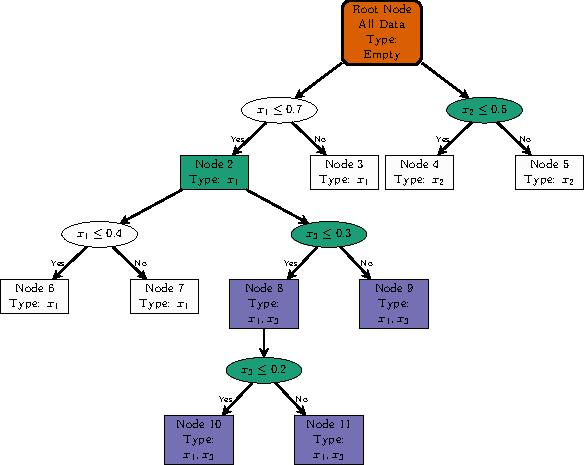
\includegraphics[width=\linewidth,height=0.75\textheight,keepaspectratio]{tree-planted-large.pdf}

}

\caption{\label{fig-planted}Planted-large}

\end{figure}%
\end{frame}

\begin{frame}{Key features of Random Planted Forests}
\phantomsection\label{key-features-of-random-planted-forests}
\begin{itemize}[<+->]
\tightlist
\item
  Ensemble of trees like RF
\item
  Splits nodes multiple times (→ \emph{non-binary} trees!)
\item
  Nodes keep track of features involved in construction
\item
  \emph{Degree of interaction} can be constrained
\item
  Prediction built incrementally using residuals (cf.~\emph{Gradient
  Boosting})
\item
  Tree stops after adjustable \emph{number of splits}
\end{itemize}
\end{frame}

\begin{frame}[fragile]{Application Example}
\phantomsection\label{application-example}
\begin{itemize}[<+->]
\tightlist
\item
  \texttt{Bikeshare} regression dataset \footnote<.->{from
    \href{https://archive.ics.uci.edu/dataset/275/bike+sharing+dataset}{UCI
    ML repository}}
\item
  Target \texttt{bikers}: Number of bikers per hour in 2011/2012
\item
  Focus on 3 features for illustration

  \begin{itemize}[<+->]
  \tightlist
  \item
    \texttt{hour} of day \(\in \{0, 1, \ldots, 23\}\)
  \item
    \texttt{temp} normalized temperature \(\in [0, 1]\)
  \item
    \texttt{workingday} \(\in\) \{\texttt{workingday},
    \texttt{no\ workingday}\}
  \end{itemize}
\item
  Average prediction: \(\hat{m}_0 \approx\) 144
\end{itemize}
\end{frame}

\begin{frame}{Main Effects}
\phantomsection\label{main-effects}
\begin{columns}[T]
\begin{column}{0.33\linewidth}
\begin{center}
\includegraphics[width=\linewidth,height=0.7\textheight,keepaspectratio]{rpf_files/figure-beamer/main-hr-1.png}
\end{center}
\end{column}

\pause

\begin{column}{0.33\linewidth}
\begin{center}
\includegraphics[width=\linewidth,height=0.7\textheight,keepaspectratio]{rpf_files/figure-beamer/main-temp-1.png}
\end{center}
\end{column}

\pause

\begin{column}{0.33\linewidth}
\begin{center}
\includegraphics[width=\linewidth,height=0.7\textheight,keepaspectratio]{rpf_files/figure-beamer/main-workingday-1.png}
\end{center}
\end{column}
\end{columns}

\begin{center}

$\hat{m} = \hat{m}_0 + \hat{m}_{\texttt{hr}}(\texttt{hr}) + \hat{m}_{\texttt{temp}}(\texttt{temp}) + \hat{m}_{\texttt{workingday}}(\texttt{workingday}) + \ldots$

\end{center}
\end{frame}

\begin{frame}{Hour \(\times\) Working Day: ``Rush Hour Effect''}
\phantomsection\label{hour-times-working-day-rush-hour-effect}
\begin{center}
\includegraphics[width=\linewidth,height=0.67\textheight,keepaspectratio]{rpf_files/figure-beamer/twoway-hr-workingday-1.png}
\end{center}

\begin{center}

$\ldots + \hat{m}_{\texttt{hr}, \texttt{workingday}}(\texttt{hr}, \texttt{workingday}) + \ldots$

\end{center}
\end{frame}

\begin{frame}{More 2nd Order Interactions}
\phantomsection\label{more-2nd-order-interactions}
\begin{columns}[T]
\begin{column}[c]{0.5\linewidth}
\begin{center}
\includegraphics[width=\linewidth,height=0.63\textheight,keepaspectratio]{rpf_files/figure-beamer/twoway-temp-workingday-1.png}
\end{center}

\(+ \hat{m}_{\texttt{temp}, \texttt{workingday}}(\texttt{temp}, \texttt{workingday})\)
\end{column}

\pause

\begin{column}[c]{0.5\linewidth}
\begin{center}
\includegraphics[width=\linewidth,height=0.63\textheight,keepaspectratio]{rpf_files/figure-beamer/twoway-hr-temp-1.png}
\end{center}

\(+ \hat{m}_{\texttt{hr}, \texttt{temp}}(\texttt{hr}, \texttt{temp}) + \ldots\)
\end{column}
\end{columns}
\end{frame}

\begin{frame}{3rd Order Interaction}
\phantomsection\label{rd-order-interaction}
\begin{center}
\includegraphics[width=\linewidth,height=0.775\textheight,keepaspectratio]{rpf_files/figure-beamer/threeway-hr-temp-woringday-1.png}
\end{center}
\end{frame}

\begin{frame}{Feature Importance in RPF}
\phantomsection\label{feature-importance-in-rpf}
\[\mathrm{FI}_S = \frac{1}{n} \sum_{i=1}^n |\hat{m}_S(\mathbf{x}_i)|\]

\begin{itemize}[<+->]
\tightlist
\item
  Average of absolute terms \(\hat{m}_S\) for \(S\) of interest
\item
  Scores also \emph{per interaction} term
\item
  Importance scores on \emph{same scale} as prediction
\end{itemize}
\end{frame}

\begin{frame}{Feature Importance: All Terms}
\phantomsection\label{feature-importance-all-terms}
\begin{center}
\includegraphics[width=\linewidth,height=0.72\textheight,keepaspectratio]{rpf_files/figure-beamer/vi-plot-thresh-1.png}
\end{center}
\end{frame}

\begin{frame}{No Free Lunch}
\phantomsection\label{no-free-lunch}
\begin{center}
(↑) Gains in interpretability \(\Rightarrow\) (↓) sacrifices in
predictive performance?

\end{center}

\vfill

\pause

\begin{itemize}[<+->]
\tightlist
\item
  Benchmark on \textbf{28} datasets \footnote<.->{OpenML-CTR23
    regression benchmark suite: \textcite{fischer2023openmlctr}}
  comparing RPF with \emph{XGBoost} \& \emph{RF}
\item
  → RPF never best, rarely bad, usually close to XGBoost
\item
  RPF slower (especially with large data)
\end{itemize}
\end{frame}

\begin{frame}{Benchmark Results (Selected Tasks)}
\phantomsection\label{benchmark-results-selected-tasks}
\begin{columns}[T]
\begin{column}{0.5\linewidth}
\begin{center}
\includegraphics[width=\linewidth,height=0.75\textheight,keepaspectratio]{rpf_files/figure-beamer/bm-scores-sel-1-1.png}
\end{center}
\end{column}

\pause

\begin{column}{0.5\linewidth}
\begin{center}
\includegraphics[width=\linewidth,height=0.75\textheight,keepaspectratio]{rpf_files/figure-beamer/bm-scores-sel-2-1.png}
\end{center}
\end{column}
\end{columns}
\end{frame}

\begin{frame}{Summary}
\phantomsection\label{summary}
\begin{center}
\textbf{Random Planted Forests} = Additive Random Forests

\end{center}

\pause

\vfill

\begin{itemize}[<+->]
\tightlist
\item
  (↑) Feature \emph{importance} on same scale as target
\item
  (↑) \emph{Main-} and \emph{interaction effects}
\item
  (↑) R package available \footnote<.->{\href{https://github.com/PlantedML/randomPlantedForest}{github.com/PlantedML/randomPlantedForest}}
\item
  (→) Competetive predictive performance (mostly)
\item
  (↓) Slower for large data (Optimization WIP!)
\end{itemize}
\end{frame}

%%% Final slide with contact information
\thanksframe{Thank you for your attention!}

%%% bib?
\begin{frame}[allowframebreaks]{References}
  \printbibliography[heading=none]
\end{frame}

\end{document}
